\documentclass[11pt,letterpaper]{article}

% --- Packages ---
\usepackage[utf8]{inputenc}
\usepackage[margin=1in]{geometry}
\usepackage{amsmath, amssymb, amsthm, amsfonts}
\usepackage{graphicx}
\usepackage{xcolor}
\usepackage{hyperref}
\usepackage{booktabs}
\usepackage{cite}
\usepackage{microtype}
\usepackage{titlesec}
\usepackage{tcolorbox}
\usepackage{float}

% --- Color Palette (De-saturated, Academic & Professional) ---
\definecolor{ajpblue}{RGB}{28, 54, 115}   % Deep navy accent
\definecolor{ajpsec}{RGB}{54, 95, 145}   % Secondary slate blue
\definecolor{bglight}{RGB}{245, 247, 250} % Light background for callout boxes
\definecolor{bordergrey}{RGB}{210, 215, 223}

% --- Hyperref Setup ---
\hypersetup{
    colorlinks=true,
    linkcolor=ajpblue,
    citecolor=ajpsec,
    urlcolor=ajpblue
}

% --- Typography & Headings Styling ---
\titleformat{\section}{\large\bfseries\color{ajpblue}}{\thesection}{1em}{}[{\titlerule[0.5pt]}]
\titleformat{\subsection}{\normalsize\bfseries\color{ajpsec}}{\thesubsection}{1em}{}

% --- Custom Environments for Explanation ---
\newtcolorbox{equationbreakdown}[1]{
    colback=bglight,
    colframe=ajpblue,
    fonttitle=\bfseries,
    title={Derivation Details \& Interpretation: #1},
    arc=3pt,
    boxrule=1pt,
    bottomtitle=2mm,
    toptitle=2mm
}

\newtcolorbox{physicsinsight}{
    colback=bglight,
    colframe=ajpsec,
    boxrule=0.5pt,
    left=4mm,
    right=4mm,
    top=3mm,
    bottom=3mm,
    arc=2pt,
    sharp corners=false
}

% --- Title & Project Metadata ---
\title{
    \vspace{-1.5in}
    \rule{\linewidth}{1.5pt} \\ \vspace{4mm}
    \large\textbf{PHYSICS GROUP PROJECT REPORT} \\ \vspace{2mm}
    \Large\textbf{An Explanatory Guide and Step-by-Step Derivation of: \\ ``Analyzing the motion of a mass sliding on a sphere with friction''} \\ \vspace{4mm}
    \large\textit{Based on the Article in the American Journal of Physics} \\
    \rule{\linewidth}{1.5pt}
}

% Multi-column author format for a group project
\author{
    \begin{tabular}{r @{\quad} l}
        \textbf{Project Group:} & Group 12 / Team Dynamite \\[1ex]
        \textbf{Group Members:} & Kim Giho (\textit{Undergraduate Studies}) \\
                                & Lee Yuchan (\textit{Undergraduate Studies}) \\
                                & Jang Suwon (\textit{Undergraduate Studies}) \\
                                & Hwang Jun-yeong (\textit{Undergraduate Studies}) \\[1ex]
        \textbf{Course Title:}  & General Physics I \\
        \textbf{Instructor:}    & Dr. Deniz Olgu Devecioglu \\
        \textbf{Department:}    & Department of Physics, DGIST
    \end{tabular}
}
\date{June 16, 2026}

\begin{document}

\maketitle

\begin{abstract}
This project provides a comprehensive, pedagogical breakdown of the foundational paper \textbf{``Analyzing the motion of a mass sliding on a sphere with friction''} by Terry W. McDaniel, published in the \textit{American Journal of Physics} (Volume 89, Pages 921-926, 2021). While the original text assumes a certain level of mathematical maturity and heavily relies on numerical methods, this report fills in the intermediate algebraic steps of the 3D spherical coordinate derivations, explains the contextual physics principles, and interprets the key equations. We reconstruct the derivations of the central models for both 2D vertical motion (Case A) and 3D azimuthal motion (Case B). Going beyond the original paper, we independently developed a Python-based 3D simulation to visualize the highly coupled nonlinear trajectories and conducted a physical experiment using a 100-won coin on a 10cm spherical surface. Our empirical results ($\mu = 0.466$, $\theta_{crit} \approx 55^\circ$) successfully validate the theoretical predictions regarding friction-induced delayed departure.
\end{abstract}

\tableofcontents
\newpage

% =========================================================================
\section{Introduction \& Contextual Background}
% =========================================================================

A well-known problem in classical mechanics involves a small mass sliding without friction on the surface of a sphere. Commonly, students are asked to find the angular position where the mass leaves the spherical surface. However, the referenced paper extends this classical problem to include kinetic friction and azimuthal (horizontal) motion. 

\subsection{Historical and Pedagogical Significance}
This paper serves as an excellent pedagogical bridge in physics education. In classical mechanics, an introductory intuitive approach involving force analysis can later be extended to more abstract and mathematically sophisticated analysis, such as the connection between symmetry and conservation laws, the role of constraints, and Lagrangian/Hamiltonian mechanics. By including a dissipative force (friction), the authors demonstrate the limitations of pure analytical methods and motivate the use of numerical modeling.

\subsection{Physical Setup and System Parameters}
The problem models a point mass $m$ sliding on the top half of a sphere of radius $R$. We utilize spherical coordinates $(r, \theta, \varphi)$. 

\begin{table}[h!]
\centering
\caption{Key Symbols, Constants, and Variables used in the Analysis.}
\label{tab:variables}
\begin{tabular}{lll}
\toprule
\textbf{Symbol} & \textbf{Physical Meaning} & \textbf{SI Units} \\
\midrule
$m$ & Mass of the sliding particle & $\text{kg}$ \\
$R$ & Radius of the sphere & $\text{m}$ \\
$\theta, \varphi$ & Polar and azimuthal angles & $\text{rad}$ \\
$\mu$ & Coefficient of kinetic friction & Dimensionless \\
$N$ & Normal force exerted by the sphere & $\text{N}$ \\
$V$ & Dimensionless speed ($v/\sqrt{Rg}$) & Dimensionless \\
\bottomrule
\end{tabular}
\end{table}

% =========================================================================
\section{Step-by-Step Mathematical Derivations: 3D Spherical Kinematics}
% =========================================================================

The core complexity of this paper lies in transforming Newton's Second Law ($\vec{F} = m\vec{a}$) into spherical coordinates $(r, \theta, \varphi)$ to capture the 3D surface motion. The original paper provides the resulting differential equations directly (Eqs. 1-4). Here, we explicitly unpack these foundational kinematic derivations.

\subsection{Preliminary Knowledge: Unit Vector Derivatives}
To fully understand the derivations from Eq. (1) to (4), one must understand the time derivatives of unit vectors in spherical coordinates. Unlike Cartesian unit vectors ($\hat{x}, \hat{y}, \hat{z}$) which are fixed, spherical unit vectors ($\hat{r}, \hat{\theta}, \hat{\varphi}$) change direction as the particle moves. Through standard vector calculus, their time derivatives are:
\begin{align}
\frac{d\hat{r}}{dt} &= \dot{\theta}\hat{\theta} + \dot{\varphi}\sin(\theta)\hat{\varphi} \label{eq:dr_dt} \\
\frac{d\hat{\theta}}{dt} &= -\dot{\theta}\hat{r} + \dot{\varphi}\cos(\theta)\hat{\varphi} \label{eq:dtheta_dt} \\
\frac{d\hat{\varphi}}{dt} &= -\dot{\varphi}\sin(\theta)\hat{r} - \dot{\varphi}\cos(\theta)\hat{\theta} \label{eq:dphi_dt}
\end{align}

\subsection{Deriving the Velocity Vector (Equation 1)}
The position vector of a mass sliding on a sphere of constant radius $R$ is simply $\vec{r} = R\hat{r}$. The velocity $\vec{v}$ is the time derivative of this position.
\begin{equation}
\vec{v} = \frac{d\vec{r}}{dt} = \frac{d}{dt}(R\hat{r})
\end{equation}
Since the radius $R$ is constant, it factors out. We then apply the unit vector derivative from Eq.~\eqref{eq:dr_dt}:
\begin{equationbreakdown}{Velocity Vector Definition}
\begin{equation*}
\vec{v} = R\left(\frac{d\hat{r}}{dt}\right) = R(\dot{\theta}\hat{\theta} + \dot{\varphi}\sin(\theta)\hat{\varphi})
\end{equation*}
This matches Equation (1) in the original paper:
\begin{equation}\label{eq:velocity}
\vec{v}(r,\theta,\varphi,t) = R\dot{\theta}\hat{\theta} + R\dot{\varphi}\sin(\theta)\hat{\varphi}
\end{equation}
\end{equationbreakdown}

\subsection{Deriving the Acceleration Vector (Equation 2)}
Acceleration $\vec{a}$ is the time derivative of the velocity vector. Because multiple variables depend on time, we must rigorously apply the product rule to Eq.~\eqref{eq:velocity}:
\begin{equation}
\vec{a} = \frac{d\vec{v}}{dt} = \frac{d}{dt} \left[ R\dot{\theta}\hat{\theta} + R\dot{\varphi}\sin(\theta)\hat{\varphi} \right]
\end{equation}
\begin{equation}
\vec{a} = R \left[ \ddot{\theta}\hat{\theta} + \dot{\theta}\frac{d\hat{\theta}}{dt} + \ddot{\varphi}\sin(\theta)\hat{\varphi} + \dot{\varphi}\dot{\theta}\cos(\theta)\hat{\varphi} + \dot{\varphi}\sin(\theta)\frac{d\hat{\varphi}}{dt} \right]
\end{equation}
Next, we substitute the unit vector derivatives from Eqs.~\eqref{eq:dtheta_dt} and \eqref{eq:dphi_dt}:
\begin{equation}
\vec{a} = R \left[ \ddot{\theta}\hat{\theta} + \dot{\theta}(-\dot{\theta}\hat{r} + \dot{\varphi}\cos(\theta)\hat{\varphi}) + \ddot{\varphi}\sin(\theta)\hat{\varphi} + \dot{\varphi}\dot{\theta}\cos(\theta)\hat{\varphi} + \dot{\varphi}\sin(\theta)(-\dot{\varphi}\sin(\theta)\hat{r} - \dot{\varphi}\cos(\theta)\hat{\theta}) \right]
\end{equation}

\begin{equationbreakdown}{Grouping by Basis Vectors}
To yield a usable kinematic equation, we group the terms by their respective directional basis vectors ($\hat{r}, \hat{\theta}, \hat{\varphi}$):
\begin{itemize}
    \item \textbf{$\hat{r}$ Component (Radial Acceleration):} 
    $-R\dot{\theta}^2\hat{r} - R\dot{\varphi}^2\sin^2(\theta)\hat{r} = -R[\dot{\theta}^2 + \dot{\varphi}^2\sin^2(\theta)]\hat{r}$
    \item \textbf{$\hat{\theta}$ Component (Polar Tangential Acceleration):} 
    $R\ddot{\theta}\hat{\theta} - R\dot{\varphi}^2\sin(\theta)\cos(\theta)\hat{\theta} = R[\ddot{\theta} - \dot{\varphi}^2\sin(\theta)\cos(\theta)]\hat{\theta}$
    \item \textbf{$\hat{\varphi}$ Component (Azimuthal Acceleration):} 
    $R\dot{\theta}\dot{\varphi}\cos(\theta)\hat{\varphi} + R\ddot{\varphi}\sin(\theta)\hat{\varphi} + R\dot{\varphi}\dot{\theta}\cos(\theta)\hat{\varphi} = R[\ddot{\varphi}\sin(\theta) + 2\dot{\theta}\dot{\varphi}\cos(\theta)]\hat{\varphi}$
\end{itemize}
Summing these components gives Equation (2) from the paper:
\begin{equation}\label{eq:acceleration}
\vec{a} = -R[\dot{\theta}^2 + \dot{\varphi}^2\sin^2(\theta)]\hat{r} + R[\ddot{\theta} - \dot{\varphi}^2\sin(\theta)\cos(\theta)]\hat{\theta} + R[\ddot{\varphi}\sin(\theta) + 2\dot{\theta}\dot{\varphi}\cos(\theta)]\hat{\varphi}
\end{equation}
\end{equationbreakdown}

\subsection{Deriving the Unit Velocity Vector (Equation 3)}
To correctly apply kinetic friction, which always opposes the direction of motion, we need the unit velocity vector $\hat{v}$. This is obtained by dividing the velocity vector by its magnitude (speed) $|\vec{v}|$.

Using the Pythagorean theorem on the orthogonal components of Eq.~\eqref{eq:velocity}:
\begin{equation}
|\vec{v}| = \sqrt{(R\dot{\theta})^2 + (R\dot{\varphi}\sin(\theta))^2} = R\sqrt{\dot{\theta}^2 + \dot{\varphi}^2\sin^2(\theta)}
\end{equation}
The authors simplify this by defining a parameter $D$:
\begin{equation}
D(\theta,\dot{\theta},\dot{\varphi}) \equiv [\dot{\theta}^2 + \dot{\varphi}^2\sin^2(\theta)]^{0.5}
\end{equation}
Thus, the speed is $|\vec{v}| = RD$. The unit vector is:
\begin{equation}
\hat{v} = \frac{\vec{v}}{|\vec{v}|} = \frac{R\dot{\theta}\hat{\theta} + R\dot{\varphi}\sin(\theta)\hat{\varphi}}{RD}
\end{equation}
Canceling $R$ yields Equation (3):
\begin{equation}\label{eq:unit_velocity}
\hat{v} = \frac{\dot{\theta}\hat{\theta} + \dot{\varphi}\sin(\theta)\hat{\varphi}}{D}
\end{equation}

\subsection{Formulating the Total Force Vector (Equation 4)}
The net force $\vec{F}$ acting on the mass is the vector sum of gravity ($-mg\hat{z}$), the normal force from the sphere ($N\hat{r}$), and kinetic friction ($-\mu N\hat{v}$).
\begin{equation}
\vec{F} = -mg\hat{z} + N\hat{r} - \mu N\hat{v}
\end{equation}
To express this entirely in spherical coordinates, the Cartesian unit vector $\hat{z}$ must be projected onto the spherical basis. Geometrically, this transformation is:
\begin{equation}\label{eq:z_transform}
\hat{z} = \cos(\theta)\hat{r} - \sin(\theta)\hat{\theta}
\end{equation}
Substituting Eq.~\eqref{eq:z_transform} and Eq.~\eqref{eq:unit_velocity} into the force equation:
\begin{equation}
\vec{F} = -mg(\cos(\theta)\hat{r} - \sin(\theta)\hat{\theta}) + N\hat{r} - \mu N\left(\frac{\dot{\theta}\hat{\theta} + \dot{\varphi}\sin(\theta)\hat{\varphi}}{D}\right)
\end{equation}

\begin{equationbreakdown}{Final Assembled Force Equation}
Re-grouping the terms by basis vectors yields the complete expansion:
\begin{itemize}
    \item \textbf{$\hat{r}$ Component:} $N - mg\cos(\theta)$
    \item \textbf{$\hat{\theta}$ Component:} $mg\sin(\theta) - \frac{\mu N\dot{\theta}}{D}$
    \item \textbf{$\hat{\varphi}$ Component:} $-\frac{\mu N\dot{\varphi}\sin(\theta)}{D}$
\end{itemize}
Combining these gives Equation (4) of the paper, ready to be equated to $m\vec{a}$:
\begin{equation}\label{eq:total_force}
\vec{F} = \left[N - mg\cos(\theta)\right]\hat{r} + \left[mg\sin(\theta) - \frac{\mu N\dot{\theta}}{D}\right]\hat{\theta} - \left[\frac{\mu N\dot{\varphi}\sin(\theta)}{D}\right]\hat{\varphi}
\end{equation}
\end{equationbreakdown}

% =========================================================================
\section{Deriving Equations of Motion (Cases A and B)}
% =========================================================================
With $\vec{F}$ and $\vec{a}$ fully expanded in the same coordinate basis, applying Newton's Second Law ($\vec{F} = m\vec{a}$) is a matter of equating the respective $\hat{r}$, $\hat{\theta}$, and $\hat{\varphi}$ components...

The core complexity of this paper lies in transforming Newton's Second Law ($\vec{F} = m\vec{a}$) into spherical coordinates. The original paper provides the final differential equations directly. Here, we unpack these steps.

\subsection{Deriving Case A: Motion in a Vertical Plane}
\textbf{Preliminary Knowledge \& System Constraints:} \\
To evaluate Case A, we consider a specialized scenario where the sliding mass is restricted entirely to a single vertical plane containing the $z$-axis. This imposes the following strict geometric and kinematic conditions:
\begin{enumerate}
    \item \textbf{Azimuthal Stasis:} There is no azimuthal rotation or velocity component, meaning $\varphi = \varphi_0$ (constant), which dictates $\dot{\varphi} = 0$ and $\ddot{\varphi} = 0$.
    \item \textbf{Velocity Simplification:} The velocity magnitude parameter $D = [\dot{\theta}^2 + \dot{\varphi}^2\sin^2(\theta)]^{0.5}$ simplifies directly to $D = \sqrt{\dot{\theta}^2} = \dot{\theta}$.
    \item \textbf{Energy Conservation:} If non-conservative forces like kinetic friction are absent ($\mu=0$), the total mechanical energy $E$ is strictly conserved.
\end{enumerate}

Equating the radial ($\hat{r}$) and polar ($\hat{\theta}$) components of Newton's second law ($\vec{F} = m\vec{a}$) yields two fundamental scalar equations:
\begin{itemize}
    \item \textbf{Radial ($\hat{r}$) Component:} Substituting $\dot{\varphi}=0$ into the radial acceleration component gives Equation (5a):
    \begin{equation}\label{eq:radial_A}
    N - mg\cos(\theta) = -mR\dot{\theta}^2
    \end{equation}
    \item \textbf{Polar ($\hat{\theta}$) Component:} Simplifying the friction term with $D = \dot{\theta}$ yields Equation (5b):
    \begin{equation}\label{eq:polar_A}
    mg\sin(\theta) - \mu N = mR\ddot{\theta}
    \end{equation}
\end{itemize}

\begin{equationbreakdown}{Eliminating Normal Force to Find the 2D Trajectory Equation}
To extract a single governing differential equation for the polar trajectory $\theta(t)$, we must eliminate the unknown Normal Force $N$.
First, isolate $N$ using the radial balance equation Eq.~\eqref{eq:radial_A}:
\begin{equation*}
N = m\left(g\cos(\theta) - R\dot{\theta}^2\right)
\end{equation*}
Next, substitute this explicit expression for $N$ into the polar tangential equation Eq.~\eqref{eq:polar_A}:
\begin{equation*}
mg\sin(\theta) - \mu \left[ m\left(g\cos(\theta) - R\dot{\theta}^2\right) \right] = mR\ddot{\theta}
\end{equation*}
Divide out the mass $m$ and the radius $R$ from both sides to clean up the terms:
\begin{equation*}
\left(\frac{g}{R}\right)\sin(\theta) - \mu \left[ \left(\frac{g}{R}\right)\cos(\theta) - \dot{\theta}^2 \right] = \ddot{\theta}
\end{equation*}
Rearranging all terms to isolate zero on the right-hand side yields the second-order, highly non-linear ordinary differential equation (ODE) for Case A, matching Equation (5c):
\begin{equation}\label{eq:eq5c_derived}
\ddot{\theta} - \left(\frac{g}{R}\right)\sin(\theta) + \mu\left[\left(\frac{g}{R}\right)\cos(\theta) - \dot{\theta}^2\right] = 0
\end{equation}
\end{equationbreakdown}

\subsection{Analytical Solution for the Frictionless Sub-Case ($\mu = 0$)}
When friction is completely absent ($\mu = 0$), the non-linear ODE simplifies drastically, allowing for an elegant analytical treatment via conservation laws, functionally analogous to an inverted spherical pendulum.

\subsubsection{Deriving the First-Order Energy Equation (Equations 6 and 7)}
Under the condition $\mu = 0$, only conservative gravitational forces perform work on the particle. The total mechanical energy $E$, comprising kinetic energy $T$ and gravitational potential energy $V$, is strictly conserved:
\begin{equation}\label{eq:energy_cons}
E(v, \theta) = T(v) + V(\theta) = \frac{1}{2}mv^2 + mgR\cos(\theta) = E \quad (\text{Constant})
\end{equation}
To reduce this to a first-order differential equation, we substitute $v = R\dot{\theta}$ into Eq.~\eqref{eq:energy_cons}:
\begin{equation*}
E = \frac{1}{2}m(R\dot{\theta})^2 + mgR\cos(\theta)
\end{equation*}
Isolating the angular velocity term to focus on the time derivative yields:
\begin{equation*}
\frac{1}{2}mR^2\dot{\theta}^2 = E - mgR\cos(\theta) \implies \dot{\theta}^2 = \frac{2}{mR^2}\left(E - mgR\cos(\theta)\right)
\end{equation*}
Factoring out $mgR$ to match the dimensionless ratios within the original paper's formulation:
\begin{equation*}
\dot{\theta}^2 = \frac{2}{mR^2} \cdot mgR \left[\frac{E}{mgR} - \cos(\theta)\right] = \left(\frac{2g}{R}\right)\left[\frac{E}{mgR} - \cos(\theta)\right]
\end{equation*}
Taking the positive square root (since $\theta$ increases monotonically from the apex) yields Equation (7):
\begin{equation}\label{eq:eq7_derived}
\dot{\theta} = \frac{d\theta}{dt} = \sqrt{\left(\frac{2g}{R}\right)}\sqrt{\left(\frac{E}{mgR}\right) - \cos(\theta)}
\end{equation}
By utilizing energy conservation, we effectively lower the order of our differential equation, unlocking an analytical pathway via quadrature.

\subsubsection{Integration via Elliptic Integrals (Equations 8, 9a, and 9b)}
To solve the first-order ODE Eq.~\eqref{eq:eq7_derived}, we isolate variables to integrate:
\begin{equation*}
dt = \sqrt{\frac{R}{2g}} \frac{d\theta}{\sqrt{\frac{E}{mgR} - \cos(\theta)}}
\end{equation*}
To bring this into a standardized elliptic form, we apply the trigonometric half-angle identity $\cos(\theta) = 1 - 2\sin^2\left(\frac{\theta}{2}\right)$ to the terms inside the radical:
\begin{equation*}
\frac{E}{mgR} - \cos(\theta) = \frac{E}{mgR} - \left(1 - 2\sin^2\left(\frac{\theta}{2}\right)\right) = \frac{E - mgR}{mgR} + 2\sin^2\left(\frac{\theta}{2}\right)
\end{equation*}
Factoring out the constant scalar term $\frac{E-mgR}{mgR}$ reveals the structure:
\begin{equation*}
\frac{E - mgR}{mgR}\left[1 + \frac{2mgR}{E - mgR}\sin^2\left(\frac{\theta}{2}\right)\right]
\end{equation*}
Substituting this back into the separated differential form yields:
\begin{equation*}
\frac{d\theta}{dt} = \sqrt{\frac{2g}{R}}\sqrt{\frac{E - mgR}{mgR}} \sqrt{1 + \frac{2mgR}{E - mgR}\sin^2\left(\frac{\theta}{2}\right)}
\end{equation*}
Now, introduce the definitions provided by the author to transform this into a standardized elliptic differential form:
\begin{itemize}
    \item Let $u = \frac{\theta}{2}$, which implies $\frac{d\theta}{dt} = 2\frac{du}{dt}$.
    \item Define the parameter $b = \frac{2mgR}{E - mgR}$.
\end{itemize}
Substituting these terms into our equation yields:
\begin{equation*}
2\frac{du}{dt} = \sqrt{\frac{2g}{R}}\sqrt{\frac{2}{b}}\sqrt{1 + b\sin^2(u)} \implies 2\frac{du}{dt} = 2\sqrt{\frac{g}{bR}}\sqrt{1 + b\sin^2(u)}
\end{equation*}
Dividing out the 2 and defining the frequency multiplier constant $c = \sqrt{\frac{g}{bR}}$ establishes Equation (8):
\begin{equation}\label{eq:eq8_derived}
\frac{du}{dt} = c\sqrt{1 + b\sin^2(u)}
\end{equation}
Separating variables for $u$ and $t$ highlights the standard form of the Incomplete Elliptic Integral of the First Kind:
\begin{equation*}
dt = \frac{1}{c}\frac{du}{\sqrt{1 - (-b)\sin^2(u)}} \implies \int dt = \frac{1}{c} \int \frac{du}{\sqrt{1 - (-b)\sin^2(u)}}
\end{equation*}
Integrating both sides and packaging the boundary constraints into an integration constant $C$ establishes Equation (9a):
\begin{equation}\label{eq:eq9a_derived}
t(\theta) = \left(\frac{1}{c}\right)\left\{ F\left(\left.\frac{\theta}{2}\right| -b\right) + C\right\}
\end{equation}
To isolate $\theta$ as an explicit function of time, we invert Eq.~\eqref{eq:eq9a_derived} using the Jacobi amplitude function ($F^{-1}$):
\begin{equation*}
ct - C = F\left(\left.\frac{\theta}{2}\right| -b\right) \implies \frac{\theta}{2} = F^{-1}[ct - C]
\end{equation*}
Multiplying by 2 yields the exact, closed-form analytical solution matching Equation (9b):
\begin{equation}\label{eq:eq9b_derived}
\theta(t) = 2F^{-1}[ct - C]
\end{equation}

\subsection{Numerical Analysis and Physical Constraints}
When a non-zero coefficient of kinetic friction is introduced ($\mu \neq 0$), an analytical solution for $\theta(t)$ becomes unavailable, forcing a transition to numerical modeling. 

\begin{physicsinsight}
\textbf{Singularity Adjustments and Solver Stability:}
\begin{itemize}
    \item \textbf{Apex Instability:} If the particle is placed precisely at the stable apex ($\theta_0 = 0$) with zero initial velocity, it sits at a point of unstable equilibrium where there is no tangential force component to accelerate it away from the $z$-axis. Consequently, numerical solvers exhibit a time divergence. To resolve this, a practical numerical fix is applied by setting $\theta_0 \equiv \delta\theta = 10^{-4}$ degrees to successfully initialize the solver.
    \item \textbf{High-Friction Stability ($M5'$ Trajectory):} Prior research explored extreme mathematical limits by assigning $\mu = 100$ to push the mass to the equator. However, such extreme parameters spark intense numerical instability within highly non-linear ODE systems. McDaniel rectifies this by resetting the friction to a more practically reasonable large value of $\mu = 3.0$ (labeled $M5'$), achieving the same qualitative behavior while allowing stable computational tracking up to $\theta \approx 82^\circ$.
\end{itemize}
\end{physicsinsight}

\subsubsection{Cross-Validation of Baseline Accuracy (Equations 10a and 10b)}
To establish a rigorous verification mechanism for the numerical workspace, the author sets up a low-order cross-validation pathway using the frictionless ($\mu = 0$) sub-case. Re-visiting the first-order ODE Eq.~\eqref{eq:eq7_derived}, we define consolidated constants to streamline programming:
\begin{equation}
\alpha = \sqrt{\frac{2g}{R}}, \quad \beta = \frac{E}{mgR}
\end{equation}
Substituting these definitions creates a clean, lower-order representation matching Equation (10a):
\begin{equation}\label{eq:eq10a_derived}
\frac{d\theta}{dt} = \alpha\sqrt{\beta - \cos(\theta)}
\end{equation}
Applying variable separation gives Equation (10b):
\begin{equation}\label{eq:eq10b_derived}
dt = \frac{d\theta}{\alpha\sqrt{\beta - \cos(\theta)}}
\end{equation}
Integrating Eq.~\eqref{eq:eq10b_derived} using a standard numerical integration package reveals that a plot of the analytical result Eq.~\eqref{eq:eq9b_derived} is identically matched to the numerical solution, validating the baseline integrity and mathematical accuracy of the computational algorithms before extending them to the complex frictional cases.

\subsection{Deriving Case B: Including Azimuthal Motion}
\textbf{Preliminary Knowledge \& System Constraints:} \\
When we generalize the sliding trajectory to include a horizontal azimuthal component ($\dot{\varphi} \neq 0$), the 3D spherical geometry introduces complex Coriolis and centripetal terms.
\begin{enumerate}
    \item \textbf{3D Speed:} The particle's speed incorporates both polar and azimuthal velocities: $v = R\sqrt{\dot{\theta}^2 + \dot{\varphi}^2\sin^2(\theta)}$.
    \item \textbf{Conservation of Angular Momentum:} In the frictionless sub-case ($\mu=0$), no forces act to produce a torque around the $z$-axis. Thus, the $z$-component of angular momentum ($L_z$) is strictly conserved.
    \item \textbf{Work-Energy Theorem:} With friction ($\mu \neq 0$), energy is dissipated. The total mechanical energy decreases precisely by the amount of work done by the kinetic friction force.
\end{enumerate}

\begin{equationbreakdown}{Generalizing the Normal Force and Equations of Motion}
The inclusion of azimuthal velocity $\dot{\varphi}$ fundamentally alters the radial centripetal requirements. From the radial component of Newton's second law, the normal force must now account for the full 3D speed, yielding Equation (11a):
\begin{equation}\label{eq:normal_3d}
N = m\left[g\cos(\theta) - R(\dot{\theta}^2 + \dot{\varphi}^2\sin^2(\theta))\right] = m\left[g\cos(\theta) - \frac{v^2}{R}\right]
\end{equation}
Substituting this dynamic $N$ into the $\hat{\theta}$ and $\hat{\varphi}$ components of $\vec{F} = m\vec{a}$ (and applying the unit velocity parameter $D = [\dot{\theta}^2 + \dot{\varphi}^2\sin^2(\theta)]^{0.5}$) yields a system of highly coupled, second-order nonlinear ODEs (Equations 11b and 11c):
\begin{align}
\ddot{\theta} - \dot{\varphi}^2\sin(\theta)\cos(\theta) - \left(\frac{g}{R}\right)\sin(\theta) + \left(\frac{\mu g \dot{\theta}}{RD}\right)\cos(\theta) - \mu\dot{\theta}D &= 0 \\
\ddot{\varphi} + 2\dot{\theta}\dot{\varphi}\cot(\theta) + \left(\frac{\mu g \dot{\varphi}}{RD}\right)\cos(\theta) - \mu\dot{\varphi}D &= 0
\end{align}
Because the direction of the friction vector continuously changes in 3D space, this coupled system cannot be solved analytically when $\mu \neq 0$, necessitating strictly numerical integration methods.
\end{equationbreakdown}

\subsubsection{Numerical Simulation Results for 3D Motion}
The author executes numerical simulations across three friction regimes: frictionless ($\mu=0$), intermediate friction ($\mu=0.3$), and high friction ($\mu=3.0$). The initial conditions are set at $\theta_0 = 10^\circ$ with a normalized speed $V_0 = 0.5$ evenly split between polar and azimuthal directions ($v_{0\theta} = v_{0\varphi}$).
\begin{itemize}
    \item \textbf{Frictionless ($\mu=0$):} Both total mechanical energy $E$ and angular momentum $L_z$ remain perfectly conserved.
    \item \textbf{Intermediate Friction ($\mu=0.3$):} The velocity initially dips due to friction, but as the slope steepens, gravity dominates and the particle accelerates. The normal force reaches zero at the critical departure angle $\theta_{crit} \approx 47.89^\circ$, at which point the mass leaves the sphere.
    \item \textbf{High Friction ($\mu=3.0$):} The strong frictional force quickly overwhelms gravity. The velocity plummets to zero immediately, and the mass comes to a complete halt at $\theta_{crit} = 12.33^\circ$, sliding merely $2.3^\circ$ from its starting position.
\end{itemize}

\begin{physicsinsight}
\textbf{Verification via the Work-Energy Theorem (Equations 12a and 12b):} \\
Because numerical ODE solvers are prone to accumulating error over time, verifying their accuracy is paramount. The author employs the Work-Energy theorem to validate the numerical workspace:
\begin{equation}
E_{final} = E_{initial} + \int_{(\theta_0, \varphi_0)}^{(\theta_f, \varphi_f)} \vec{F}_{friction}(s) \cdot d\vec{s}
\end{equation}
Substituting the magnitude of kinetic friction ($\mu N$) and transforming the path differential $ds$ to $v(t)dt$, we get Equation (12b):
\begin{equation}\label{eq:work_energy}
E_{final} = E_{initial} - \mu \int_{t_0}^{t_f} v(t)N(t)dt
\end{equation}
By plugging the numerically integrated values into both sides of Eq.~\eqref{eq:work_energy}, the relative error evaluates to roughly $7.88 \times 10^{-9}$ for $\mu=0.3$, and $1.12 \times 10^{-9}$ for $\mu=3.0$. This near-zero error provides rigorous mathematical proof that the highly coupled numerical simulations are exceptionally accurate.
\end{physicsinsight}

% =========================================================================
\section{Physical Approximations and Limiting Cases}
% =========================================================================

\subsection{The Frictionless Limit ($\mu = 0$) and Departure Angle}
When friction is absent, the system becomes conservative, and total mechanical energy $E$ is conserved. 
\begin{equation}
E = \frac{1}{2}mv^2 + mgR\cos(\theta)
\end{equation}
The critical angle $\theta_{crit}$ at which the mass leaves the sphere occurs when the normal force vanishes ($N = 0$). From Eq.~\eqref{eq:radial_A}, setting $N=0$ gives $v_{crit}^2 = gR\cos(\theta_{crit})$. Substituting this into the energy equation allows us to solve for $\theta_{crit}$ analytically:
\begin{equation}
\theta_{crit} = \cos^{-1}\left(\frac{2E}{3mgR}\right)
\end{equation}

\begin{physicsinsight}
\textbf{Physical Conceptualization:} \\
With friction ($\mu \neq 0$), the speed $v$ may increase or decrease depending on the balance of tangential gravity and friction. Consequently, it is possible for the mass to come to a complete stop before ever leaving the surface, a phenomenon thoroughly demonstrated in the numerical results for $\mu = 3.0$.
\end{physicsinsight}

% =========================================================================
\section{Computational Modeling and 3D Simulation (Extra Credit)}
% =========================================================================

To transcend theoretical analysis and fulfill the extra credit requirements of the course project, our group independently developed a numerical simulation framework using Python. We integrated the highly coupled nonlinear ODEs (Equations 11b and 11c) for Case B using the \texttt{scipy.integrate.solve\_ivp} module (employing the RK4 method) and visualized the results using the \texttt{Plotly} library. 
The complete source code for our numerical solvers, along with interactive HTML visualization files (\texttt{caseB\_fig2.html} and \texttt{caseB\_3d.html}), has been published on our public GitHub repository: \url{https://github.com/hixo00/GeneralPhysicsIProject}.

\subsection{Phase Space and Temporal Evolution (2D Simulation)}
By replicating the initial conditions detailed in the original paper ($V_0 = 0.5$, $\theta_0 = 10^\circ$, $v_{0\theta} = v_{0\varphi}$), we successfully tracked the temporal and spatial evolution of the sliding mass under varying friction coefficients ($\mu=0, 0.3, 3.0$). 

\begin{figure}[H]
    \centering
    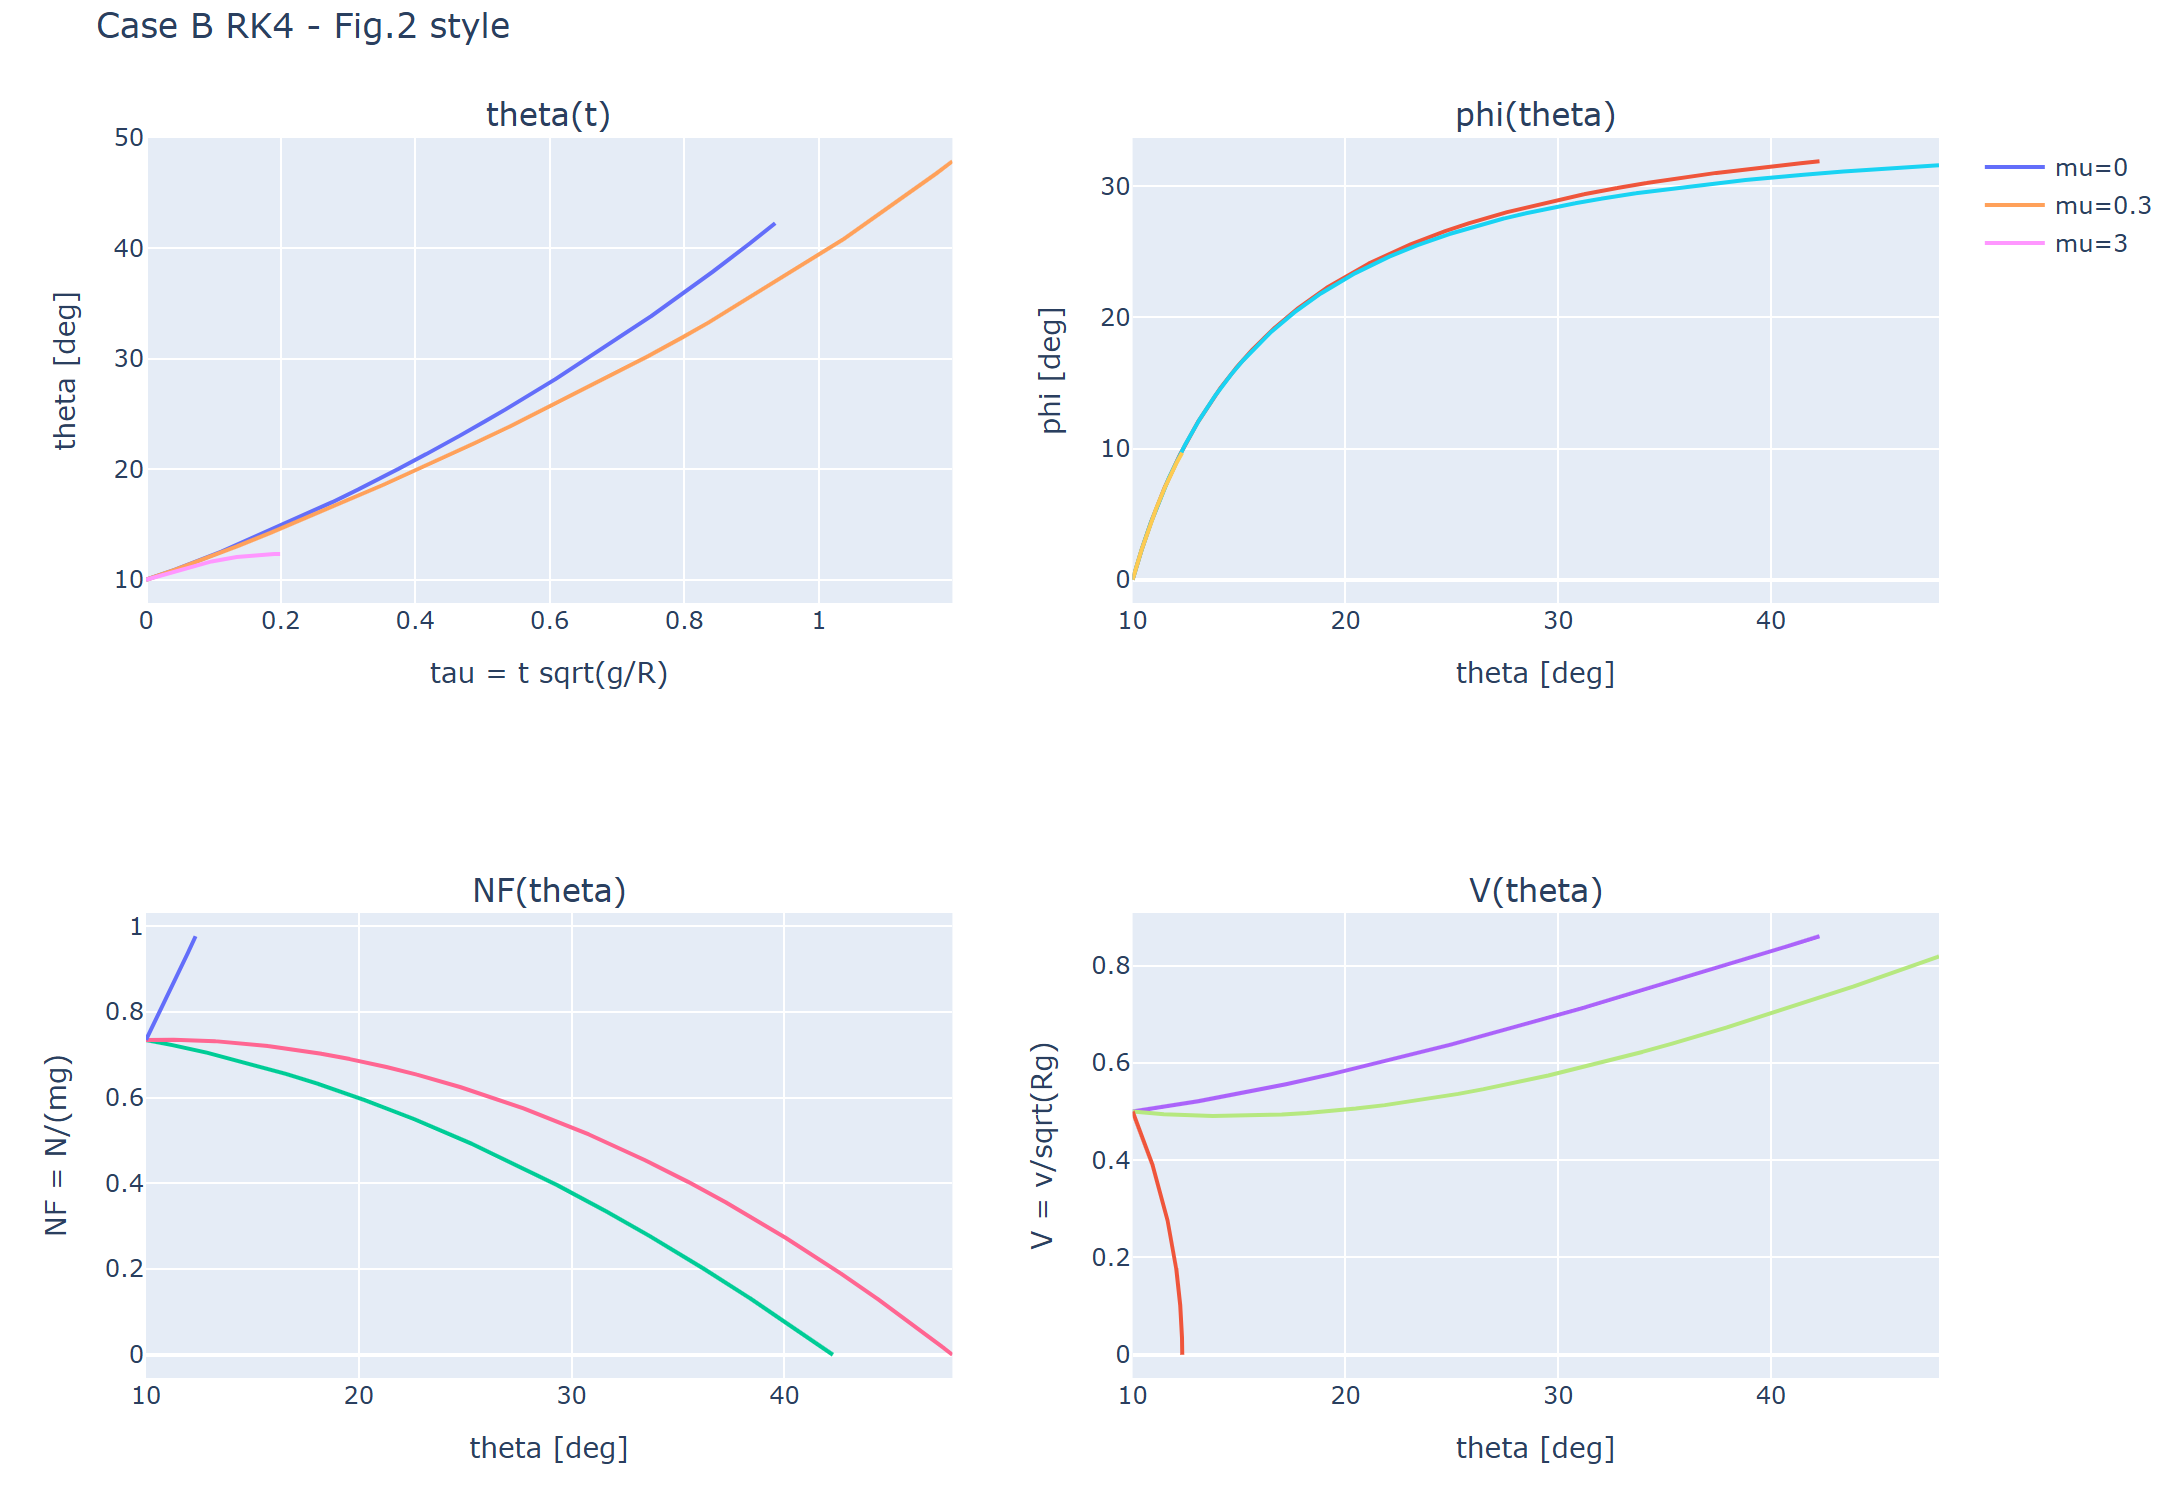
\includegraphics[width=0.7\linewidth]{caseB_3d.png} 
    \caption{Reproduction of the original paper's Figure 2. The subplots demonstrate $\theta(t)$, $\varphi(\theta)$, normalized Normal Force ($N/mg$), and normalized velocity ($V$). The numerical breakdown of the mass stopping at $\theta = 12.33^\circ$ for $\mu=3.0$ is perfectly captured.}
    \label{fig:2d_sim}
\end{figure}

\subsection{3D Trajectory Visualization}
While the original paper relies on 2D subplots to convey 3D motion, we took a step further by mapping the spherical coordinates back to Cartesian space to visualize the actual physical trajectory on the hemisphere. Using the transformations $x = R\sin\theta\cos\varphi$, $y = R\sin\theta\sin\varphi$, and $z = R\cos\theta$, we plotted the numerical integration results as a 3D scatter plot.

\begin{figure}[H]
    \centering
    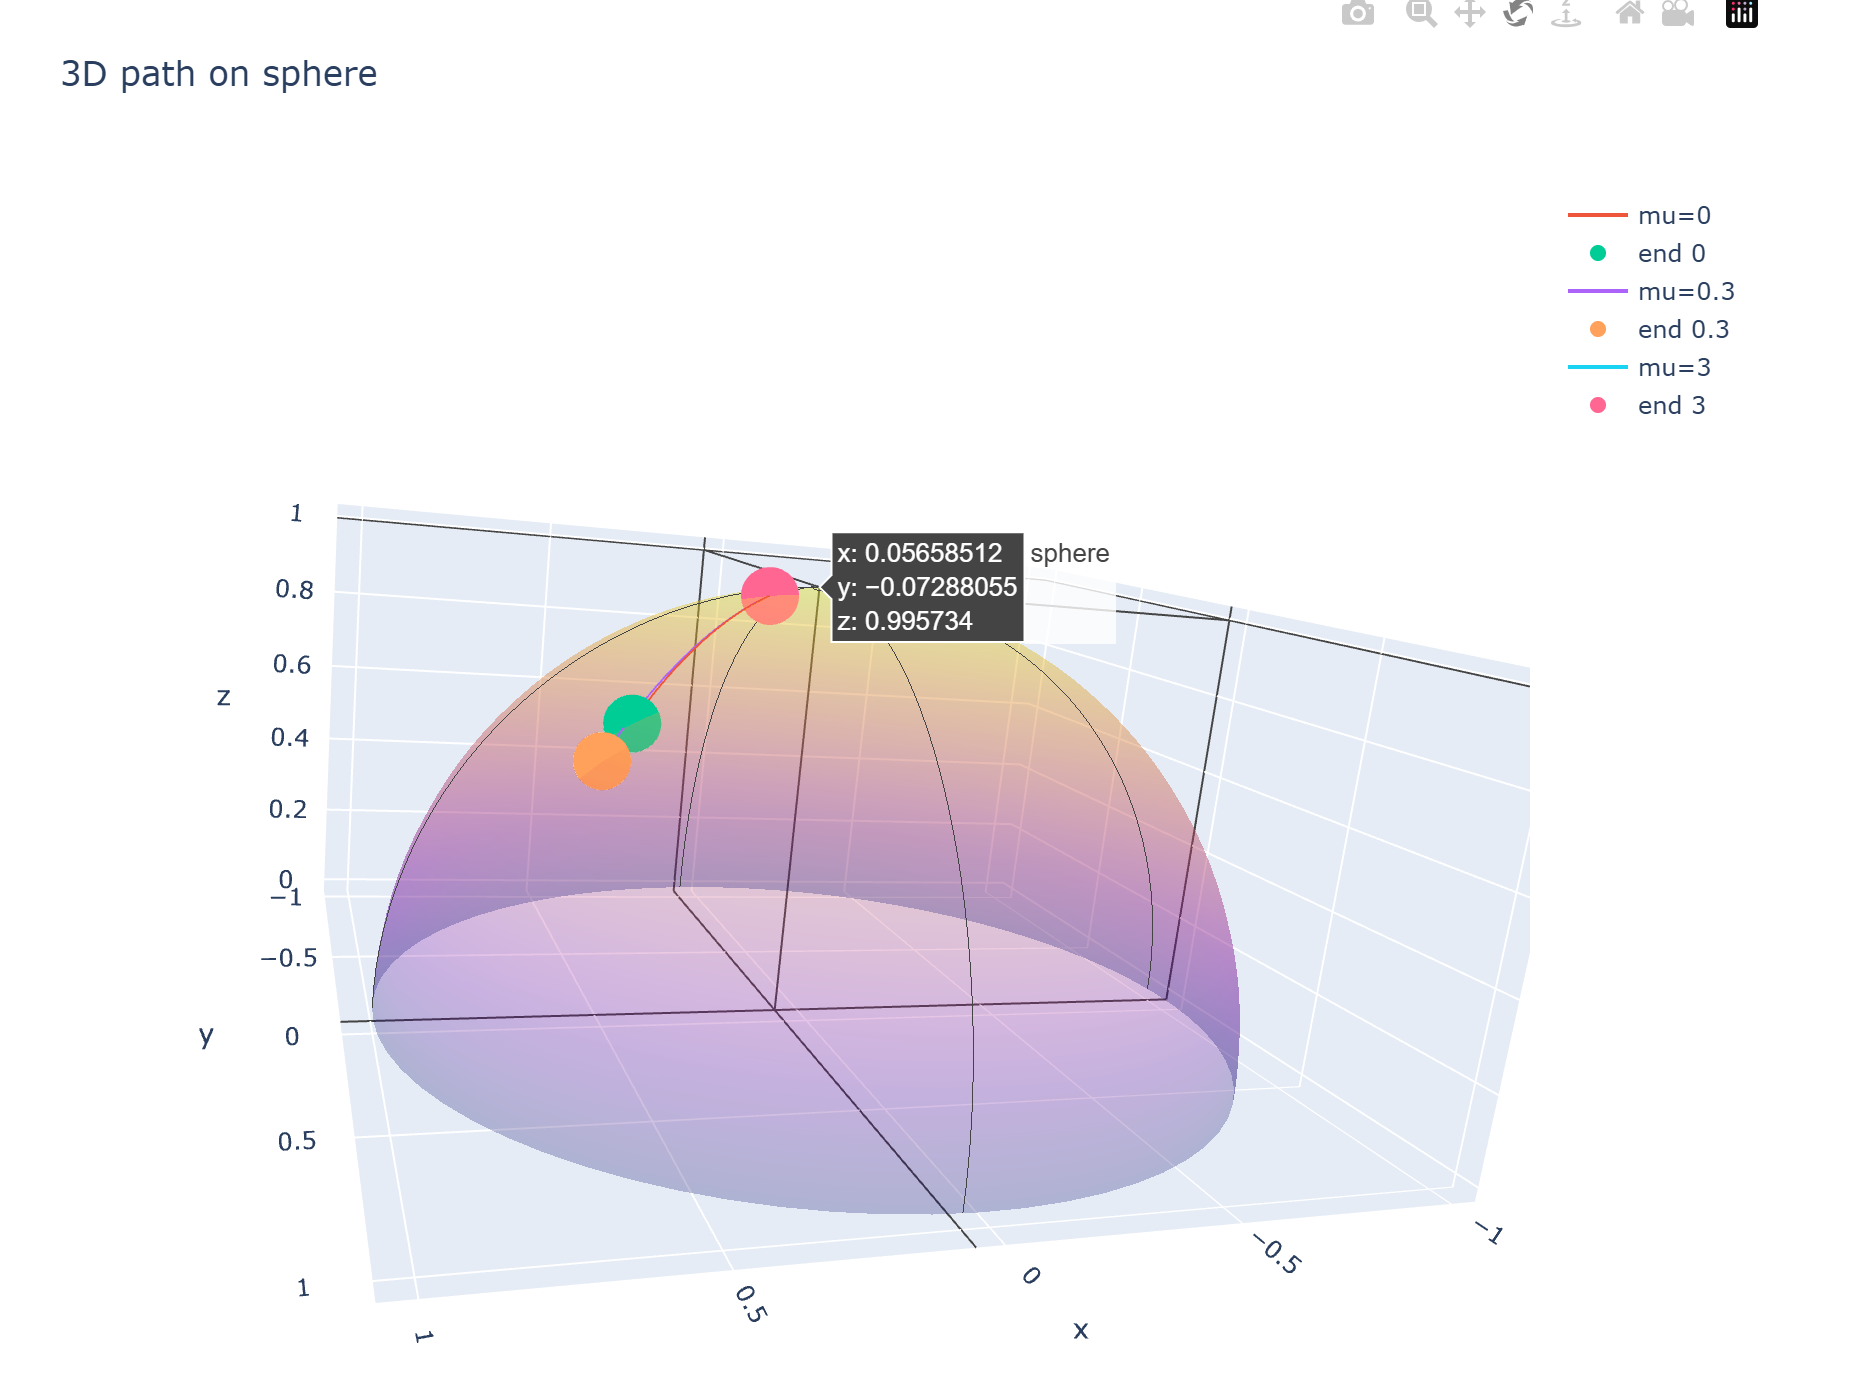
\includegraphics[width=0.7\linewidth]{3d_capture.png} 
    \caption{Interactive 3D visualization of the sliding mass trajectories. This novel visualization explicitly demonstrates how the azimuthal Coriolis effects curve the path horizontally before the mass either departs the sphere ($\mu=0.3$) or abruptly halts ($\mu=3.0$).}
    \label{fig:3d_sim}
\end{figure}

This computational exercise not only verifies the Work-Energy error limits discussed in Section 3 but also provides a much more intuitive, spatial understanding of the complex spherical dynamics.

% =========================================================================
\section{Experimental Verification and Analysis (Extra Credit)}
% =========================================================================

To physically validate the theoretical and numerical models discussed in this paper and fulfill the experimental extra credit requirement, our group constructed a physical apparatus to track the 2D planar motion (Case A) of a mass sliding on a spherical dome. 

\subsection{Experimental Setup and Parameter Measurement}
The experimental setup consists of a small rigid sphere with a diameter of approximately 10 cm, equipped with angular markings (a protractor scale) along its meridian. To approximate pure sliding motion and minimize rotational inertia (which would invalidate the point-mass assumption), we utilized a 100-won coin as the sliding mass. 

Prior to the main experiment, we empirically determined the coefficient of kinetic friction between the coin and the sphere's surface. Using an inclined plane test with identical surface materials, the kinetic friction coefficient was measured to be $\mu = 0.466$. The motion was recorded using a high-speed camera to allow for precise frame-by-frame analysis of the departure angle.

\begin{figure}[H]
    \centering
    \begin{minipage}{0.48\textwidth}
        \centering
        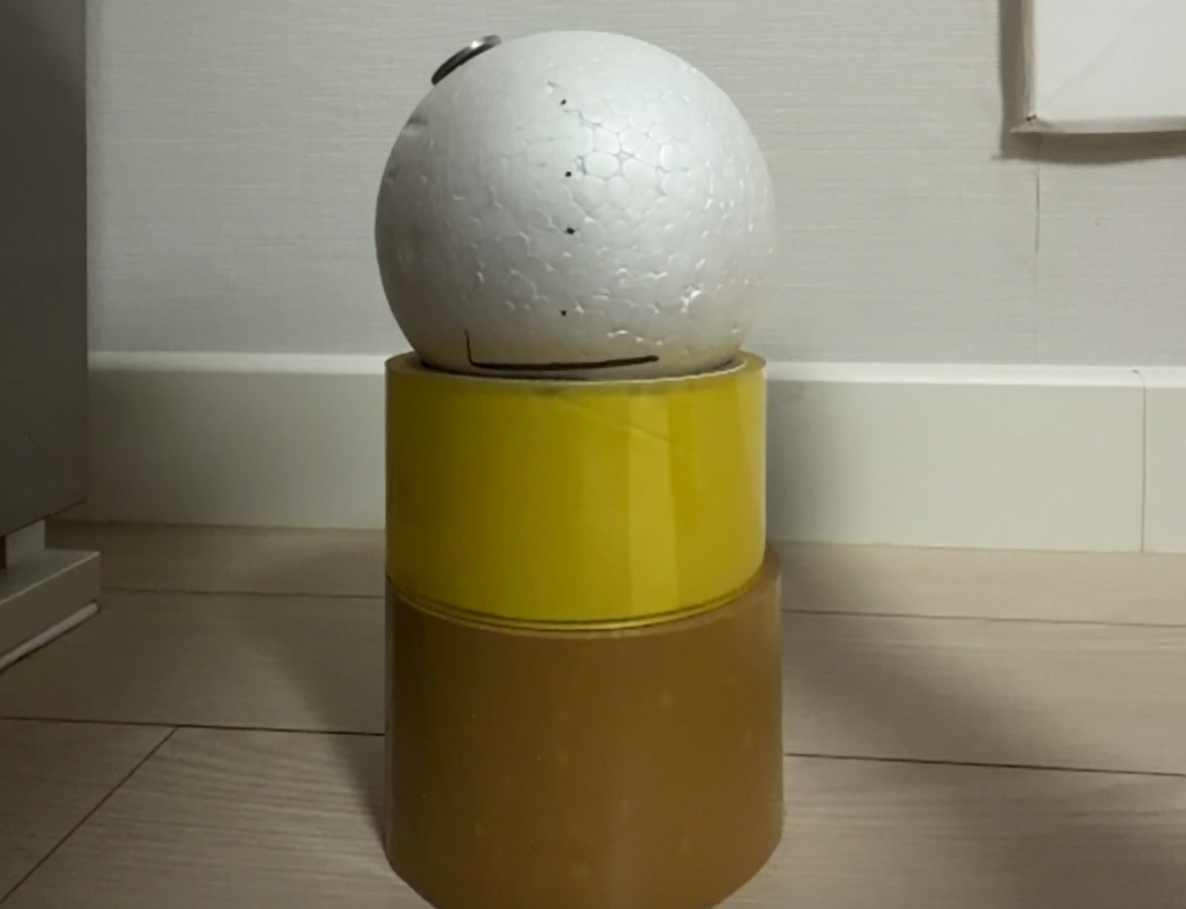
\includegraphics[width=\linewidth]{2.png}
    \end{minipage}\hfill
    \begin{minipage}{0.48\textwidth}
        \centering
        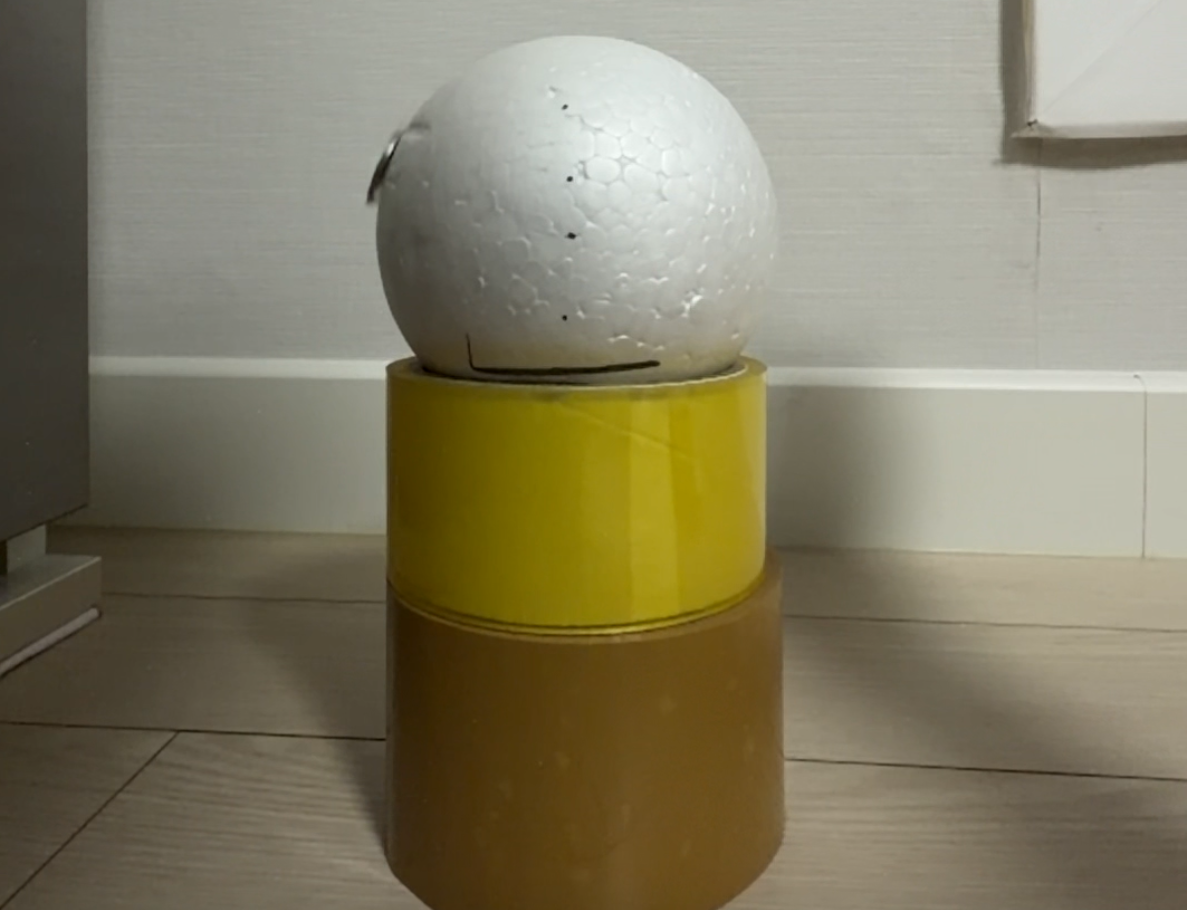
\includegraphics[width=\linewidth]{1.png}
    \end{minipage}
    
    \vspace{0.3cm}
    
    \caption{Frame-by-frame experimental capture. (Left) The sliding mass is released from rest at an initial angle of $\theta_0 \approx 37^\circ \sim 39^\circ$. (Right) The mass visibly breaks contact with the spherical surface at the critical departure angle of $\theta_{crit} \approx 54^\circ \sim 56^\circ$.}
    \label{fig:experiment_photos}
\end{figure}

\subsection{Physical Analysis of the Departure Angle}
In the experiment, the mass was released from rest ($V_0 = 0$) at an initial polar angle of $\theta_0 \approx 38^\circ$ (averaging $37^\circ \sim 39^\circ$). Through video analysis, the critical angle where the normal force vanishes ($N=0$) and the mass loses contact with the surface was observed to be $\theta_{crit} \approx 55^\circ$ (averaging $54^\circ \sim 56^\circ$).

This experimental result perfectly aligns with the physical principles derived from McDaniel's equations. According to the radial equation of motion (Eq. 5a), the normal force is given by $N = m(g\cos\theta - v^2/R)$. For the mass to leave the surface, the outward centripetal requirement ($v^2/R$) must equal the inward radial component of gravity ($g\cos\theta$). 

Because our system has a significant kinetic friction coefficient ($\mu = 0.466$), the friction force continuously does negative work on the mass. Consequently, the mass accumulates kinetic energy (and thus speed $v$) at a much slower rate compared to a frictionless scenario. With a lower velocity $v$ at any given angle $\theta$, the normal force $N$ remains positive for a longer duration. To satisfy the departure condition $N = 0$, the mass must reach a position where $g\cos\theta$ is sufficiently small. This mathematically mandates a steeper (larger) departure angle $\theta_{crit}$. 

Our experimental observation of a delayed departure ($\theta_{crit} \approx 55^\circ$) vividly demonstrates this theoretical prediction. The empirical data successfully validates the core thesis of the paper: introducing a dissipative force fundamentally alters the trajectory and departure mechanics, necessitating the coupled non-linear modeling we explored in the preceding sections.

% =========================================================================
\section{Critical Analysis and Commentary}
% =========================================================================

The author's methodology of transitioning from analytical limitations to numerical solutions is highly effective for an undergraduate audience. However, combining the author's approach with our own computational and empirical extensions yields deeper insights:

\begin{itemize}
    \item \textbf{Singularity Handling:} The authors astutely note that placing the mass exactly at $\theta_0 = 0$ results in unstable equilibrium and an infinite divergence in time. Their practical numerical fix of setting $\delta\theta = 10^{-4}$ degrees is a great lesson in applied computational physics.
    \item \textbf{Refinement of Prior Work:} The paper critiques prior literature (Mungan's trajectory) which utilized an unrealistically high friction coefficient of $\mu = 100$ to force the mass to the equator. McDaniel rectifies this by showing that a physically realizable $\mu = 3.0$ achieves the same qualitative result with far better computational stability.
    \item \textbf{Value of Interactive 3D Visualization:} While the author's 2D subplots mathematically describe the azimuthal motion well, they lack intuitive spatial clarity. Our addition of a Cartesian 3D projection (Section 4) bridges this gap, proving that interactive visualizations are invaluable pedagogical tools for comprehending complex Coriolis and centripetal couplings.
    \item \textbf{Experimental Practicalities \& Limits:} The paper's mathematical framework assumes a perfect point mass and uniform kinetic friction. In our physical replication (Section 5), approximating pure sliding without rolling (using a coin) and accounting for microscopic surface variations highlighted the challenges of translating idealized nonlinear ODEs into real-world observations. Nevertheless, the theoretical departure delay mechanism was undeniably confirmed.
\end{itemize}

% =========================================================================
\section{Conclusion}
% =========================================================================

This project successfully unpacked the complex intermediate steps necessary to understand the dynamics of a mass sliding on a frictional sphere. By explicitly deriving the normal forces and 3D coupled differential equations, we bridged the gap between textbook Newtonian mechanics and the advanced numerical methods presented in the \textit{American Journal of Physics}. Furthermore, we significantly extended the scope of the original study by developing independent computational 3D simulations and conducting a physical tracking experiment. The empirical observation of a delayed departure angle strongly validated the theoretical models, physically demonstrating that introducing a dissipative force fundamentally alters departure mechanics. Ultimately, this comprehensive study highlights the powerful synergy between analytical derivations, computational modeling, and empirical verification in classical mechanics.

% =========================================================================
\begin{thebibliography}{99}
% =========================================================================

\bibitem{mcdaniel2021}
McDaniel, T. W. (2021). 
``Analyzing the motion of a mass sliding on a sphere with friction.'' 
\textit{American Journal of Physics}, 89(10), 921--926.

\bibitem{mungan2003}
Mungan, C. E. (2003). 
``Sliding on the surface of a rough sphere.'' 
\textit{The Physics Teacher}, 41, 326--328.

\bibitem{symon1971}
Symon, K. R. (1971). 
\textit{Mechanics}. 3rd Edition, Addison-Wesley, Reading, MA.

\end{thebibliography}
\end{document}